Możliwośc zastosowania podwójnych siatek metalowych (ang. DMG - double metallic grating)\nomenclature{DMG}{ang. Double Metallic Grating - podwójna metalowa siatka dyfrkacyjna} w celu uzyskania różnej transmisji w przypadku propagacji światła w przeciwnych kierunkach przez strukturę zostało zaproponowane przez Chen Cheng i innych \cite{cheng2007controllable,cheng2008physical,xu2011unidirectional}. Budowa podwójnej siatki metalowej została przedstawiona na rysunku \ref{fig:1ddmg-schem}. Uzyskanie transmisji jednokierunkowej możliwe jest przy dobraniu parametrów układu tak, aby $\Lambda_1 = 2\Lambda_2$ oraz długość fali E-M padającej na DMG  $\lambda$ spełniała nierówność $\Lambda_2<\lambda<\Lambda_2$. Przywołując klasyczne prawo Braggów
\begin{equation}
	\Lambda \cdot \textrm{sin}(\alpha_n) = n \lambda 
\end{equation}
dla padania pod kątem $0^{\circ}$, zakładając otoczenie w postaci powietrza z obu stron DMG możemy wyprowadzić warunek na liczbę rzędów ugięcia uzyskiwanych przy użyciu siatki dyfrakcyjnej o okresie $\Lambda$. 
\begin{equation}
	 0 \le |n| \le \frac { \Lambda }{\lambda},
\end{equation}
z którego wynika, że omawiany układ może wykazywać się jednie -1,~0~i~1 rzędem ugięcia pochodzącymi od siatki o okresie $\Lambda_1$. Ze względu na podfalowy okres $\Lambda_2$ fala E-M będzie przez tę siatkę propagować się bez zmiany kierunku. Cała struktura może być traktowana jako układ sprzężający dwie siatki dyfrakcyjne, w których przesunięcie pomiędzy pomiędzy siatkami może posłużyć do regulacji zmiany fazy przed sprzężenie pola za jedną siatką do pola przed drugą\cite{marcet2008controlling}. Na skutek modyfikacji fazy, jeden z rzędów ugięcia może zostać wygaszony przez interferencję. 
	
\begin{figure}[tb]
	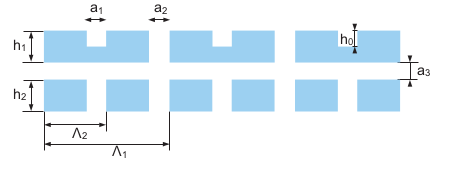
\includegraphics[width=\textwidth]{images/thz/1D-DMG-schemat.png}
	\caption{Schemat omawianej podwójnej siatki metalowej wykorzystywanej }
	\label{fig:1ddmg-schem}
\end{figure}


 Z innej perspektywy strukturę typu DMG można analizować jako układ falowodów metal-dielektryk-metal, o rozmiarach podfalowych ( $a_1,a_2,a_3 < \lambda$), dlatego wzbudzany może być w nich jedynie mod podstawowy w polaryzacji TM\footnote{Podobnie jak w  podrozdziale \ref{subart:rezo-grating}}. 

Przedstawiona struktura wykazuje asymetrię w transmisji -1~i~1 rzędu ugięcia. W przypadku oświetlenia od strony siatki o okresie $\Lambda_1$ wiązka światła zostaje transmitowana jedynie do -1~i~1 rzędu ugięcia, ze względu na interferencyjne wygaszenie rzędu 0. Następnie w sposób nie zmodyfikowany jest transmitowana przez siatkę o charakterze podfalowym $\Lambda_2$. Gęstość energii pola E-M odpowiadająca opisanej sytuacji została przedstawiona na rysunku \ref{fig:trans_gora}. 
	Przy oświetleniu z przeciwnej strony różnica w fazie składowych dochodzących do szczelin w siatce wyjściowej wynosi $\pi$ na skutek czego wewnątrz falowodów struktury dochodzi do destruktywnej interferencji i fala E-M nie jest transmitowana. Odpowiedni rozkład gęstości energii pola E-M prezentuje rysunek \ref{fig:trans_dol}. W wyniku optymalizacji numerycznej parametrów struktury uzyskano znaczącą różnicę we współczynniku transmisji w przypadku oświetlenia z różnych stron DMG dla szerokiego spektrum długości fali. Zależność współczynnika transmisji przez DMG w przeciwnych kierunkach w zależności od długości fali przedstawia wykres na rysunku \ref{fig:tran_freq}.


\begin{figure}
	\begin{subfigure}{0.9\textwidth}
		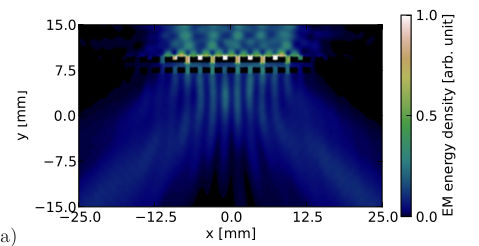
\includegraphics[width=\textwidth]{images/thz/opt_lett_gora.png}
		\label{fig:trans_gora}
	\end{subfigure}

	\begin{subfigure}{0.9\textwidth}
		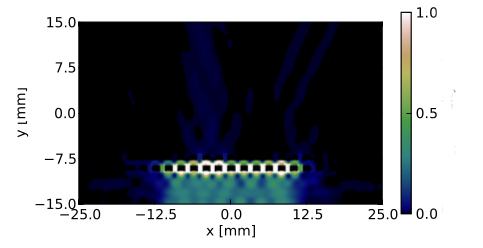
\includegraphics[width=\textwidth]{images/thz/opt_letters_dol.png}
		\label{fig:trans_dol}
	\end{subfigure}
	\caption{Rozkład gęstości energi pola E-M w przypadku prostopadłego oświetlenia układu DMG z różnych stron. }
	\label{fig:tras_gora_dol}
\end{figure}

\begin{figure}	
	\centering
	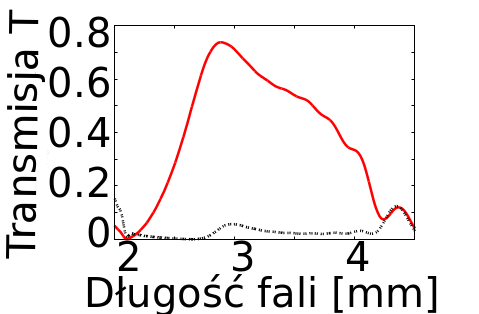
\includegraphics[width=0.5\textwidth]{images/thz/opt_lett_spect.png}
	\caption{Zależność współczynnika transmisji przez omawianą strukturę DMG od długości fali dla oświetlenia z różnych stron. Wykres odpowiada DMG o $\Lambda_1= 2 \Lambda_2 = 4.2$~mm, $a_1=a_2=a_3=0.7$~mm, $h_1=h_2=2 h_0=1$~mm.}
	\label{fig:trans_freq}

\end{figure}
